% !TEX encoding = UTF-8 Unicode
\documentclass[a4paper]{article}

\usepackage{color}
\usepackage{url}
\usepackage{amsmath}
\usepackage{csquotes}
\usepackage[T2A]{fontenc} % enable Cyrillic fonts
\usepackage[utf8]{inputenc} % make weird characters work
\usepackage{graphicx}
\usepackage{fullwidth}

\usepackage[english,serbian]{babel}
%\usepackage[english,serbianc]{babel} %ukljuciti babel sa ovim opcijama, umesto gornjim, ukoliko se koristi cirilica

\usepackage[unicode]{hyperref}
\hypersetup{colorlinks,citecolor=green,filecolor=green,linkcolor=blue,urlcolor=blue}

\usepackage{listings}
\usepackage{verbatim}
% \usepackage{pseudocode}
\usepackage{algorithm}
\usepackage{algorithmic}
%\newtheorem{primer}{Пример}[section] %ćirilični primer
\newtheorem{primer}{Primer}[section]

\definecolor{mygreen}{rgb}{0,0.6,0}
\definecolor{mygray}{rgb}{0.5,0.5,0.5}
\definecolor{mymauve}{rgb}{0.58,0,0.82}



% my commands
\newcommand{\q}[1]{``#1''}  %use this command for quoting
\newcommand{\s}[0]{\textit{s}} %use this for italic s
\newcommand{\sstar}[0]{$\textit{s}^*$}
\newcommand{\squote}[0]{$\textit{s}^\prime$}
\renewcommand{\S}[0]{$\mathcal{S}$} %use this for instead of $\mathcal{S}$
\newcommand{\Sstar}[0]{$\mathcal{S}^{*}$}
\newcommand{\eng}[1]{(\textit{eng.} #1)}
\newcommand{\lokalna}[0]{\small{\texttt{LokalnaPretraga}}}
\newcommand{\kriterijum}[0]{\small{\texttt{KriterijumPrihvatanja}}}
\newcommand{\generisi}[0]{\small{\texttt{GenerišiPočetnoRešenje}}}
\newcommand{\perturbacija}[0]{\small{\texttt{Perturbacija}}}
\floatname{algorithm}{Algoritam}



\lstset{ 
  backgroundcolor=\color{white},   % choose the background color; you must add \usepackage{color} or \usepackage{xcolor}; should come as last argument
  basicstyle=\scriptsize\ttfamily,        % the size of the fonts that are used for the code
  breakatwhitespace=false,         % sets if automatic breaks should only happen at whitespace
  breaklines=true,                 % sets automatic line breaking
  captionpos=b,                    % sets the caption-position to bottom
  commentstyle=\color{mygreen},    % comment style
  deletekeywords={...},            % if you want to delete keywords from the given language
  escapeinside={\%*}{*)},          % if you want to add LaTeX within your code
  extendedchars=true,              % lets you use non-ASCII characters; for 8-bits encodings only, does not work with UTF-8
  firstnumber=1000,                % start line enumeration with line 1000
  frame=single,	                   % adds a frame around the code
  keepspaces=true,                 % keeps spaces in text, useful for keeping indentation of code (possibly needs columns=flexible)
  keywordstyle=\color{blue},       % keyword style
  language=Python,                 % the language of the code
  morekeywords={*,...},            % if you want to add more keywords to the set
  numbers=left,                    % where to put the line-numbers; possible values are (none, left, right)
  numbersep=5pt,                   % how far the line-numbers are from the code
  numberstyle=\tiny\color{mygray}, % the style that is used for the line-numbers
  rulecolor=\color{black},         % if not set, the frame-color may be changed on line-breaks within not-black text (e.g. comments (green here))
  showspaces=false,                % show spaces everywhere adding particular underscores; it overrides 'showstringspaces'
  showstringspaces=false,          % underline spaces within strings only
  showtabs=false,                  % show tabs within strings adding particular underscores
  stepnumber=2,                    % the step between two line-numbers. If it's 1, each line will be numbered
  stringstyle=\color{mymauve},     % string literal style
  tabsize=2,	                   % sets default tabsize to 2 spaces
  title=\lstname                   % show the filename of files included with \lstinputlisting; also try caption instead of title
}

\begin{document}

\title{Iterativna lokalna pretraga\\ \small{Seminarski rad u okviru kursa\\Metodologija stručnog i naučnog rada\\ Matematički fakultet}}

\author{Aleksa Voštić, Lazar Perišić, Anđela Križan, Anđela Janošević\\ akile9v@gmail.com, lakiwow95@gmail.com,\\ endzikri@gmail.com, andjelaj197@gmail.com}

%\date{9.~april 2015.}

\maketitle

%%%%%%%%%%%%%%%%%%%%%%%%%%%%%%%%%%%%%%%%%%%%%%%%%%%%%%%%%%%%%%%%%%%%%%%%%%%%%%%%%%%%%%%%%%%%%%%%%%%%%%%%%%%%%%%%%
%%%%%%%%%%%%%%%%%%%%%%%%%%%%%%%%%%%%%%%%%%%%%%%%%%%%%%%%%%%%%%%%%%%%%%%%%%%%%%%%%%%%%%%%%%%%%%%%%%%%%%%%%%%%%%%%%
% Pocetak dela (za menjanje pitati autora ovog dela)
% autor: Lazar Perisic
%%%%%%%%%%%%%%%%%%%%%%%%%%%%%%%%%%%%%%%%%%%%%%%%%%%%%%%%%%%%%%%%%%%%%%%%%%%%%%%%%%%%%%%%%%%%%%%%%%%%%%%%%%%%%%%%%
%%%%%%%%%%%%%%%%%%%%%%%%%%%%%%%%%%%%%%%%%%%%%%%%%%%%%%%%%%%%%%%%%%%%%%%%%%%%%%%%%%%%%%%%%%%%%%%%%%%%%%%%%%%%%%%%%

\abstract{Osnovna ideja ove metaheuristike je da se pretraga fokusira na samo deo mogućih rešenja koja dobija od ugrađene heuristike. 
Iako jednostavna zbog svoje modularnosti, pokazuje odlične rezultate u praksi. U radu je prikazana njena implementacija, kao i pristup kojim se došlo do nje. 
Takođe, prikazane su neke od primena ovog algoritma.}

%%%%%%%%%%%%%%%%%%%%%%%%%%%%%%%%%%%%%%%%%%%%%%%%%%%%%%%%%%%%%%%%%%%%%%%%%%%%%%%%%%%%%%%%%%%%%%%%%%%%%%%%%%%%%%%%%
%%%%%%%%%%%%%%%%%%%%%%%%%%%%%%%%%%%%%%%%%%%%%%%%%%%%%%%%%%%%%%%%%%%%%%%%%%%%%%%%%%%%%%%%%%%%%%%%%%%%%%%%%%%%%%%%%
% Kraj dela (za menjanje pitati autora ovog dela)
% autor: Lazar Perisic
%%%%%%%%%%%%%%%%%%%%%%%%%%%%%%%%%%%%%%%%%%%%%%%%%%%%%%%%%%%%%%%%%%%%%%%%%%%%%%%%%%%%%%%%%%%%%%%%%%%%%%%%%%%%%%%%%
%%%%%%%%%%%%%%%%%%%%%%%%%%%%%%%%%%%%%%%%%%%%%%%%%%%%%%%%%%%%%%%%%%%%%%%%%%%%%%%%%%%%%%%%%%%%%%%%%%%%%%%%%%%%%%


\tableofcontents

\newpage
%%%%%%%%%%%%%%%%%%%%%%%%%%%%%%%%%%%%%%%%%%%%%%%%%%%%%%%%%%%%%%%%%%%%%%%%%%%%%%%%%%%%%%%%%%%%%%%%%%%%%%%%%%%%%%%%%
% Pocetak dela (za menjanje pitati autora ovog dela)
% autor: Anđela Janošević
%%%%%%%%%%%%%%%%%%%%%%%%%%%%%%%%%%%%%%%%%%%%%%%%%%%%%%%%%%%%%%%%%%%%%%%%%%%%%%%%%%%%%%%%%%%%%%%%%%%%%%%%%%%%%%%%%
\section{Uvod}
\label{sec:uvod}

Važnost algoritama visokih performansi za rešavanje teških optimizacionih problema ne može se potceniti, i u mnogim
slučajevima jedine dostupne metode su metaheuristike. Prilikom dizajniranja metaheuristike, poželjno je da bude jednostavna, i
konceptualno i u praksi. Prirodno, takođe mora biti efikasna i, ako je moguće, opšte namene. Ako metaheuristiku posmatramo kao
jednostavnu konstrukciju za usmeravanje (specifične za problem) heuristike, idealan slučaj je kada se metaheuristika može
koristiti bez ikakvog znanja o zavisnosti od problema.

Kako su metaheuristike postale sve sofisticiranije, ovaj idealan
slučaj je gurnut u stranu u potrazi za većim performansama. Kao posledica toga, znanje specifično za problem mora biti
inkorporirano u metaheuristiku da bi se dostiglo vrhunsko stanje. Nažalost, ovo čini granicu između heuristike i
metaheuristike nejasnom, i mi rizikujemo da izgubimo i jednostavnost i opštost. Da bi se suprotstavili tome, približavamo se
modularnosti i pokušavamo da dekompozitujemo metaheuristički algoritam na nekoliko delova, svaki sa svojom specifičnošću.
Konkretno, želeli bismo imati potpuno opšti namenski deo, dok bi svako znanje specifično za problem ugrađeno u metaheuristiku
bilo odvojeno u drugi deo. Konačno, u najvećoj mogućoj meri, radije ostavljamo netaknutu ugrađenu heuristiku (koju treba
\q{voditi}) zbog svoje potencijalne složenosti. \textbf{Iterativna lokalna pretraga} pruža jednostavan način da se zadovolje svi
ovi zahtevi. Suština iterativne lokalne pretrage je da se izbegne zaglavljivanje u lokalnom minimumu tako što u više iteracija primenjuje
lokalnu pretragu na novo generisano početno rešenje.

Svrha ovog rada je da se prikaže detaljan opis iterativne lokalne pretrage.
Do sada je, uprkos svojoj konceptualnoj jednostavnosi, dovela do brojnih vrhunskih rezultata bez korišćenja previše znanja
specifičnog za problem.

%%%%%%%%%%%%%%%%%%%%%%%%%%%%%%%%%%%%%%%%%%%%%%%%%%%%%%%%%%%%%%%%%%%%%%%%%%%%%%%%%%%%%%%%%%%%%%%%%%%%%%%%%%%%%%%%%
% Kraj dela (za menjanje pitati autora ovog dela)
% autor: Anđela Janošević
%%%%%%%%%%%%%%%%%%%%%%%%%%%%%%%%%%%%%%%%%%%%%%%%%%%%%%%%%%%%%%%%%%%%%%%%%%%%%%%%%%%%%%%%%%%%%%%%%%%%%%%%%%%%%%%%%







%%%%%%%%%%%%%%%%%%%%%%%%%%%%%%%%%%%%%%%%%%%%%%%%%%%%%%%%%%%%%%%%%%%%%%%%%%%%%%%%%%%%%%%%%%%%%%%%%%%%%%%%%%%%%%%%%
%%%%%%%%%%%%%%%%%%%%%%%%%%%%%%%%%%%%%%%%%%%%%%%%%%%%%%%%%%%%%%%%%%%%%%%%%%%%%%%%%%%%%%%%%%%%%%%%%%%%%%%%%%%%%%%%%
% Pocetak dela (za menjanje pitati autora ovog dela)
% autor: Lazar Perisic
%%%%%%%%%%%%%%%%%%%%%%%%%%%%%%%%%%%%%%%%%%%%%%%%%%%%%%%%%%%%%%%%%%%%%%%%%%%%%%%%%%%%%%%%%%%%%%%%%%%%%%%%%%%%%%%%%
%%%%%%%%%%%%%%%%%%%%%%%%%%%%%%%%%%%%%%%%%%%%%%%%%%%%%%%%%%%%%%%%%%%%%%%%%%%%%%%%%%%%%%%%%%%%%%%%%%%%%%%%%%%%%%%%%

\section{Ideja iza iterativne lokalne pretrage}
Pretpostavimo da imamo algoritam za specifičan problem koji aproksimira optimalno rešenje u okolini trenutnog rešenja. 
Taj algoritam ćemo zvati lokalna pretraga, iako to ne mora da bude \textit{prava} lokalna pretraga i  
izvršavaćemo ga pozivanjem procedure \lokalna{}. Pitanje koje se postavlja jeste \q{Da li 
ovaj algoritam može da se poboljša korišćenjem iteracije?}. Odgovor je da može, a rezultati dobijeni u praksi pokazuju 
da je to poboljšanje u većini situacija značajno \cite{beginnersIntroduction}.\footnotemark
\footnotetext{U retkim slučajevima kada iterativni metod nije pogodan za dati algoritam poboljšanje će biti minimalno.} 

Neka je $\mathcal{C}$ funkcija cene nekog problema optimizacije. Kao i u većini slučajeva kada se pominje funkcija cene,
tako i ovde, cilj nam je da tu funkciju minimizujemo. Potencijalna rešenja ovog problema ćemo označiti sa \s{}, 
a skup svih tih rešenja sa \S{}. Naša lokalna pretraga tj. procedura \lokalna{} definiše preslikavanje 
iz skupa \S{} u \Sstar{} koji predstavlja skup lokalno optimalnih rešenja \sstar{}.

Osnovna ideja ILS \eng{iterated local search} tj. iterativne lokalne pretrage jeste da izbegne mane pokretanja lokalne pretrage iz nasumičnih delova prostora pretrage, 
odnosno skupa \S{}. Ovako dobijena rešenja nisu međusobno zavisna i lokalnu pretragu treba pozivati na ovaj način samo kada druga rešenja ne daju bolje rezultate.\footnotemark
\footnotetext{Iako se ovo retko dešava, ovaj pristup se u tim situacijama preporučuje zbog dobiti u jednostavnosti} 
Uz to, kako se broj rešenja povećava, verovatnoća da nađemo kvalitetno \sstar{} opada, što u praksi znači da kada broj rešenja teži beskonačnosti, kvalitetno, odnosno rešenje koje je blizu optimuma (globalnog), je 
nemoguće naći \cite{handbookOfMetaheuristics}. ILS se vodi idejom da umesto da koristi sva rešenja odnosno ona iz skupa \S{}, koristi samo podskup njih, odnosno skup \Sstar{}. 
Cilj je da se krećemo kroz skup \Sstar{} i tako dođemo do globalnog optimuma ili bar rešenja bliskog njemu.
Dakle, u svakoj iteraciji imamo trenutno rešenje \sstar{} na koje vršimo perturbaciju \eng{perturbation}, odnosno pomeramo se iz njega u međustanje 
\squote{}. Ovo međustanje pripada \S{} i na njega primenjujemo \lokalna{} da bismo došli do rešenja $\textit{s}^{*\prime}$ iz \Sstar{}. Sada odlučujemo da li prihvatamo ovo rešenje i nastavljamo od njega potragu ili 
se vraćamo na prethodno \sstar{} rešenje. Ovu funkciju obezbeđuje procedura \kriterijum{}.
Iterativnu lokalnu pretragu definišemo na način prikazan u algoritmu \ref{alg:1} a grafički prikaz iste se vidi na slici \ref{figure:iterativna}.

\begin{figure}[h!]
  \centering
  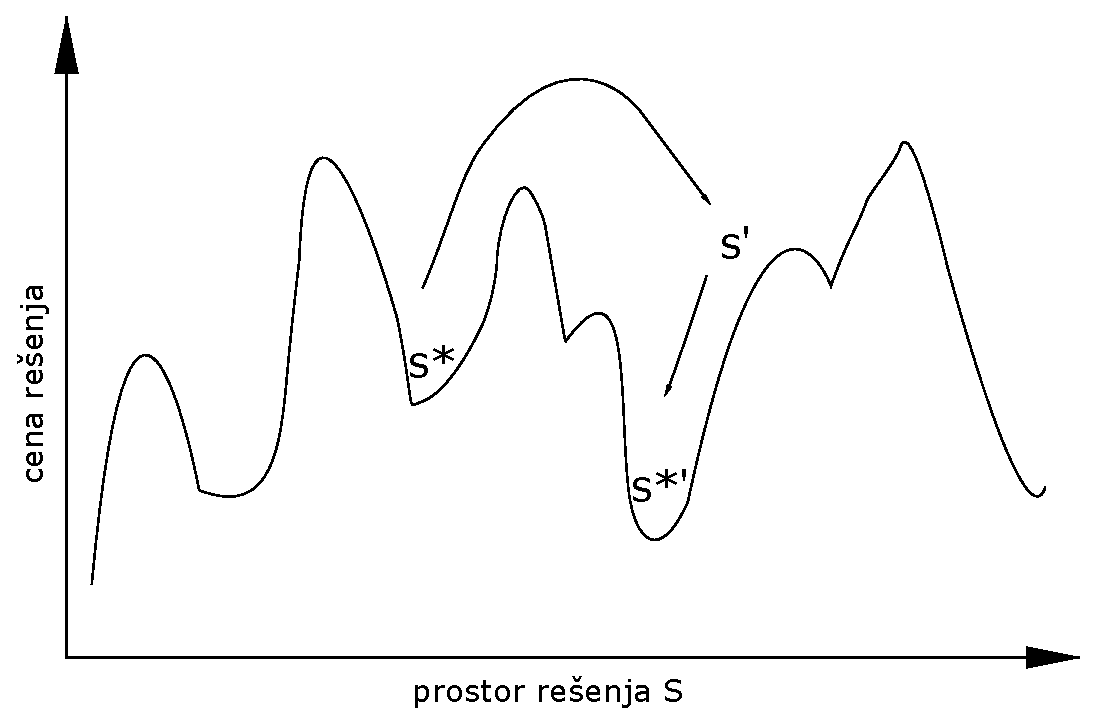
\includegraphics[width=0.8\textwidth]{slika.eps}
  \caption{Grafički prikaz ILS. Na trenutno rešenje \sstar{} primenjujemo \perturbacija{}, dobijamo \squote{} na koje primenjujemo \lokalna{} nakon čega dobijamo novo rešenje $\textit{s}^{*\prime{}}$.}
  \label{figure:iterativna}
\end{figure}


\begin{fullwidth}[width=\linewidth,leftmargin=+\textwidth/2-\linewidth/2]
\begin{algorithm}[H]
  \caption{Iterativna lokalna pretraga}
  \label{alg:1}
  \begin{algorithmic}
  \STATE $\textit{s}_0$ = \generisi{}()
  \STATE \sstar{} = \lokalna{}($\textit{s}_0$)
  \REPEAT
  \STATE \squote{} = \perturbacija{}(\sstar{}, \textit{istorija})
  \STATE $\textit{s}^{*\prime}$ = \lokalna{}(\squote{})
  \STATE \sstar{} = \kriterijum{}(\sstar{}, $\textit{s}^{*\prime}$, \textit{istorija})
  \UNTIL \textsc{nije zadovoljen uslov zaustavljanja}\footnotemark
  \RETURN \textsc{najbolje rešenje}
  \end{algorithmic}
  \end{algorithm}
\end{fullwidth}

\footnotetext{\textsc{uslov zaustavljanja} je obično dozvoljeno vreme izvršavanja programa \eng{runtime} ili broja iteracija}
\section{Implementacija iterativne lokalne pretrage}
Kao što možemo da vidimo iz prethodnog, da bismo implementirali algoritam tj. iterativnu lokalnu pretragu, 
potrebno je da implementiramo četiri komponente: \generisi{}, \lokalna{}, \perturbacija{} i \kriterijum{}. 

\subsection{Početno rešenje}

Početno rešenje može biti veoma važno, pogotovo ako nam je cilj što brži dolazak do kvalitetnih rešenja. 
Generisanje početnih rešenja se može izvesti na dva načina. Možemo da koristimo (\romannumeral 1) metodu slučajnog izbora, 
ili (\romannumeral 2) metodu pohlepne heuristike. U opštem slučaju, nije moguće reći koji metod od ova dva je bolji. Ipak, za kraća 
izvršavanja ILS preporučuje se metoda pohlepne heuristike, dok prilikom dužeg izvršavanja ILS izbor početnog rešenja nije mnogo bitan \cite{beginnersIntroduction, online}.

\subsection{Perturbacija}

Perturbacije, odnosno pomeranja su veoma važna komponenta ovog algoritma. Naime, one služe da se pobegne od lokalnih minimuma (optimalnih rešenja) koji su često 
znatno lošiji od globalnog minimuma. ILS to čini tako što primenjuje perturbaciju na trenutni lokalni minimum. Definisaćemo snagu odnosno intenzitet perturbacije 
kao broj komponenti rešenja koji je perturbacijom promenjen. Snaga perturbacije je osobina koja najviše utiče na ovu komponentu algoritma. Naime, ako je snaga previše velika 
onda će se algoritam ponašati kao prilikom pokretanja lokalne pretrage iz nasumičnih delova prostora pretrage, a ako je previše mala, lokalna pretraga će često 
poništiti perturbaciju i kao novo rešenje 
naći ono od koga je krenula. Samim tim malo novih rešenja će biti istraženo. Ova veličina varira od problema do problema, a takođe zavisi i od veličine problema. 
Ponašanje ILS u praksi pokazuje da ne postoji jedinstvena optimalna snaga perturbacije. Ona se može menjati tokom izvršavanja i tada koristimo adaptivne perturbacije. 
Jedan način da se one implementiraju jeste korišćenjem istorije pretrage. Drugi način jeste determinističkim određivanjem tokom izvršavanja \cite{handbookOfMetaheuristics, beginnersIntroduction}.

\subsection{Kriterijum prihvatanja}

Nakon što dobijemo novo moguće rešenje $\textit{s}^{*\prime}$, na osnovu procedure \kriterijum{} odlučujemo da li to rešenje prihvatamo kao novo trenutno rešenje. 
Možemo imati neki od dva ekstremna pristupa:
\begin{itemize}
  \item Uvek prihvatamo novo rešenje
  \item Ako je novo rešenje $\textit{s}^{*\prime}$ bolje od \sstar{}, onda ga prihvatamo, inače ne
\end{itemize}
Mnogi pristupi između ova dva su svakako mogući i često korišćeni. \\
\kriterijum{} ima jak uticaj na prirodu korišćenih rešenja. Naime, u kombinaciji sa \perturbacija{}, može da se 
koristi za kontrolu ravnoteže između intenzifikacije\footnote{Prihvatanjem samo boljih rešenja, smanjićemo prostor pretrage i pretraživati rešenja u trenutnoj okolini} \eng{intensification} 
i diverzifikacije\footnote{Prihvatanjem svih rešenja, povećavamo prostor pretrage i imamo veliki broj rešenja, ali često pretražujemo okoline sa lošim rešenjima} \eng{diversification}. Kao i kod perturbacije 
možemo koristiti istoriju pretrage za dinamičko određivanje kriterijuma prihvatanja \cite{handbookOfMetaheuristics, beginnersIntroduction}. 

\subsection{Lokalna pretraga}

Do sada smo lokalnu pretragu koju koristi ILS koristili kao crnu kutiju \eng{black box}. Znali smo šta ta procedura radi ali nismo ulazili u detalje implementacije. Ipak, često nam je implementacija lokalne pretrage poznata 
i to nam omogućava da dodatno optimizujemo ILS. Postoji mnogo algoritama koji mogu da se koriste kao lokalna pretraga. Može se pretpostaviti da što je bolja lokalna pretraga to je bolji ILS. To često jeste tačno, ali postoje 
situacije kada lošiji algoritam daje bolja rešenja. Jedna od tih situacije je kada imamo ograničeno vreme izvršavanja programa i tada je nekad bolje koristiti brži, u teoriji lošiji algoritam i pozvati ga mnogo više puta nego 
bolji i sporiji algoritam. Zavisno od razlike u potrebnom vremenu, možemo dozvoliti više vremena za izvršavanje i koristiti bolji algoritam. Ako razlika u brzini dva algoritma nije velika, onda je obično isplativije koristiti bolji. 
Za određene probleme, često se kao lokalna pretraga koristi metaheuristika poput tabu pretrage \eng{tabu search}, simuliranog kaljenja \eng{simulated annealing} itd \cite{handbookOfMetaheuristics}.

%%%%%%%%%%%%%%%%%%%%%%%%%%%%%%%%%%%%%%%%%%%%%%%%%%%%%%%%%%%%%%%%%%%%%%%%%%%%%%%%%%%%%%%%%%%%%%%%%%%%%%%%%%%%%%%%%
%%%%%%%%%%%%%%%%%%%%%%%%%%%%%%%%%%%%%%%%%%%%%%%%%%%%%%%%%%%%%%%%%%%%%%%%%%%%%%%%%%%%%%%%%%%%%%%%%%%%%%%%%%%%%%%%%
% Kraj dela (za menjanje pitati autora ovog dela)
% autor: Lazar Perisic
%%%%%%%%%%%%%%%%%%%%%%%%%%%%%%%%%%%%%%%%%%%%%%%%%%%%%%%%%%%%%%%%%%%%%%%%%%%%%%%%%%%%%%%%%%%%%%%%%%%%%%%%%%%%%%%%%
%%%%%%%%%%%%%%%%%%%%%%%%%%%%%%%%%%%%%%%%%%%%%%%%%%%%%%%%%%%%%%%%%%%%%%%%%%%%%%%%%%%%%%%%%%%%%%%%%%%%%%%%%%%%%%


%%%%%%%%%%%%%%%%%%%%%%%%%%%%%%%%%%%%%%%%%%%%%%%%%%%%%%%%%%%%%%%%%%%%%%%%%%%%%%%%%%%%%%%%%%%%%%%%%%%%%%%%%%%%%%%%%
%%%%%%%%%%%%%%%%%%%%%%%%%%%%%%%%%%%%%%%%%%%%%%%%%%%%%%%%%%%%%%%%%%%%%%%%%%%%%%%%%%%%%%%%%%%%%%%%%%%%%%%%%%%%%%%%%
% Pocetak dela (za menjanje pitati autora ovog dela)
% autor: Andjela Krizan
%%%%%%%%%%%%%%%%%%%%%%%%%%%%%%%%%%%%%%%%%%%%%%%%%%%%%%%%%%%%%%%%%%%%%%%%%%%%%%%%%%%%%%%%%%%%%%%%%%%%%%%%%%%%%%%%%
%%%%%%%%%%%%%%%%%%%%%%%%%%%%%%%%%%%%%%%%%%%%%%%%%%%%%%%%%%%%%%%%%%%%%%%%%%%%%%%%%%%%%%%%%%%%%%%%%%%%%%%%%%%%%%%%%
\section{Primene iterativne lokalne pretrage}
ILS algoritmi su uspešno primenjeni u raznim kombinatornim optimizacionim problemima. U određenim slučajevima ovi algoritmi dostižu veoma visoke performanse. U ovom poglavlju prikazaćemo neke najčešće probleme.
\subsection{Problem trgovackog putika}
Problem trgovačkog putnika je verovatno najpoznatiji kombinatorni optimizacijski problem. U suštini, on služi za testiranje izrade novih ideja algoritama, a dobre performanse na Problemu trgovačkog putnika se uzimaju kao dokaz vrednosti takvih ideja. Kao i mnoge metaheuristike, neki od prvih ILS algoritama su testirani na ovom problemu. 

Baum je prvi to uradio, osmislivši metodu ponovljenog spusta. On je u svojim testovima koristio tehniku 2-opt (pojava udvojenih razmena) kao ugrađenu heuristiku, nasumične 3-promene kao perturbacije, i smanjivao je dužinu obilaska (odatle je i ime ove metode). Njegovi rezultati nisu bili zadovoljavajući, delom jer je razmatrao ne-Euklidski Problem trgovačkog putnika koji je suštinski teži u praksi od Euklidskog.

LSMC (Large-step Markov chain) algoritam je doneo velika poboljšanja. Martin, Otto i Felten su u ovom algoritmu koristili simulirano kaljenje kao optimizaciju iz koje je izvedeno ime algoritma. Oni su razmotrili primenu 3-opt lokalne pretrage i Lin-Kernighan heuristike (LK) koji je najbolji algoritam lokalne pretrage za Problem trgovačkog putika. Ali, ključni momenat njihovog rada je uvođenje duplog mosta za perturbaciju, što je bilo bitno za dalji rad na Euklidskom Problemu trgovačkog putnika.

D.S.Jonhson je za ILS koristio LK kao lokalnu pretragu, i osmislio je naziv \q{iterated Lin-Kernighan} (ILK). Razlike u imlementaciji u odnosu na LSMC su:
\begin{itemize}
  \item potezi između dva mosta su nasumični
  \item cene se poboljšavaju (prihvataju se samo bolje)
\end{itemize}
Od ovih prvih studija predložene su i druge varijante ILS-a, a Johnson i McGeoch su dali sažetak stanja 1997 godine. 
ILS za Problem trgovačkog putnika sa najvišim performansama je trenutno lančani LK kodiran od strane Applegate, Bixby, Chivatal i Cook, koji su detaljno opisali implementaciju. Oni su vršili eksperimente na ovom kodu uzimajući u obzir druge module:
\begin{itemize}
  \item inicijalni obilazak
  \item izbori implementacije LK heuristike
  \item tipovi perturbacija
\end{itemize}
Njihovi testovi su vršeni na velikim instancama do čak 25 milion gradova. Za potez sa dvostrukim mostom, razmatrali su efekat forsiranja ivica da budu kratke i istraživali su nasumične poteze sa dva mosta. Oni su zaključili da se najbolje performanse postižu kada su potezi dvostukog mosta usmereni prema kratkim dužinama ivica. Međutim, jačinu usmeravanja ka kratkim ivicama treba prilagoditi raspoloživom vremenu računanja, tj. što je kraće vreme računanja, ivice bi trebalo da budu kraće. Pri testiranju uticaja inicijalnog obilaska, došli su do zaključka da najgore performanse postižu slučajni početni obilasci, dok su najbolje rezultate dali Kristofidesov algoritam i pohlepna heuristika. 

Osim ovih radova, predložena su još dva ILS algoritma za Problem trgovačkog putnika. Thomas Stützle je ispitiao ponašanje ILS algoritma za Problem trgovačkog putnika, i zaključio da ILS algoritmi stagniraju tokom dugog perioda izvođenja, što je i očekivano pri vršenju intenzivnog pretraživanja. Da bi se izbeglo stagniranje, predloženo je ponovno pokretanje i poseban kriterijum prihvatanja zbog variranja pretrage. Cilj te strategije je da prisiliti pretragu da nastavi od pozicije koja je veća od odredjenog minimalnog rastojanja od trenutne pozicije. Rezultati pokazuju da je ova metoda veoma efikasna, čak i kada se koristi samo 3-opt lokalna pretraga. 


Drugi ILS algoritam od 1997. godine su razvili Katayama i Marisha. Oni su uveli novi mehanizam perturbacije i nazvali su ga genetska transformacija. Mehanizam genetske transformacije koristi dva obilaska, jedan od njih predstavlja do sada najbolje rešenje, a drugi je obilazak koji je pronađen ranije u pretrazi. Eksperimenti sa iterativnim LK algoritmom koji koristi genetsku transformaciju umesto standardnog dvostrukog mosta pokazuju da je pristup vrlo efikasan.
%%Č č
%%Ć ć
%%Dž dž
%%Đ đ
%%Š š
%%Ž ž
%%%


%%%%%%%%%%%%%%%%%%%%%%%%%%%%%%%%%%%%%%%%%%%%%%%%%%%%%%%%%%%%%%%%%%%%%%%%%%%%%%%%%%%%%%%%%%%%%%%%%%%%%%%%%%%%%%%%%
%%%%%%%%%%%%%%%%%%%%%%%%%%%%%%%%%%%%%%%%%%%%%%%%%%%%%%%%%%%%%%%%%%%%%%%%%%%%%%%%%%%%%%%%%%%%%%%%%%%%%%%%%%%%%%%%%
% Kraj dela (za menjanje pitati autora ovog dela)
% autor: Andjela Krizan
%%%%%%%%%%%%%%%%%%%%%%%%%%%%%%%%%%%%%%%%%%%%%%%%%%%%%%%%%%%%%%%%%%%%%%%%%%%%%%%%%%%%%%%%%%%%%%%%%%%%%%%%%%%%%%%%%
%%%%%%%%%%%%%%%%%%%%%%%%%%%%%%%%%%%%%%%%%%%%%%%%%%%%%%%%%%%%%%%%%%%%%%%%%%%%%%%%%%%%%%%%%%%%%%%%%%%%%%%%%%%%%%%%%



%%%%%%%%%%%%%%%%%%%%%%%%%%%%%%%%%%%%%%%%%%%%%%%%%%%%%%%%%%%%%%%%%%%%%%%%%%%%%%%%%%%%%%%%%%%%%%%%%%%%%%%%%%%%%%%%%
%%%%%%%%%%%%%%%%%%%%%%%%%%%%%%%%%%%%%%%%%%%%%%%%%%%%%%%%%%%%%%%%%%%%%%%%%%%%%%%%%%%%%%%%%%%%%%%%%%%%%%%%%%%%%%%%%
% Pocetak dela (za menjanje pitati autora ovog dela)
% autor: Aleksa Voštić
%%%%%%%%%%%%%%%%%%%%%%%%%%%%%%%%%%%%%%%%%%%%%%%%%%%%%%%%%%%%%%%%%%%%%%%%%%%%%%%%%%%%%%%%%%%%%%%%%%%%%%%%%%%%%%%%%
%%%%%%%%%%%%%%%%%%%%%%%%%%%%%%%%%%%%%%%%%%%%%%%%%%%%%%%%%%%%%%%%%%%%%%%%%%%%%%%%%%%%%%%%%%%%%%%%%%%%%%%%%%%%%%%%%
\subsection{Problemi raspoređivanja}
ILS se takođe može uspešno primeniti i na probleme raspoređivanja kao što su Single Machine Total Weighted Tardiness Problem, Flow shop problem, Job shop scheduling problem
kao i mnogi drugi.
\subsubsection{Single Machine Total Weighted Tardiness Problem}
SMTWTP je jedan od fundimentalnih kombinatornih problema optimizacije. Naime, problem se sastoji od skupa nezavisnih poslova sa različitim vremenima obrade, težinama (cenama), kao i rokovima do kad poslovi moraju biti završeni predviđenim da se obrađuju na jednoj datoj mašini. Ideja je minimalizovati ukupno kašnjenje sa datim težinskim koeficijentima čija je uloga da kvantifikuju važnost svakog posla ili označi troškove kašnjenja izvršavanja posla na mašini, odnosno utvrditi optimalan redosled izvršavanja ovih poslova na jednoj mašini.


ILS algoritam za rešavanje ovog problema zasnovan je na osnovu dinamičke pretrage, odnosno koristi tehnike dinamičkog programiranja kako bi pronašao najbolji potez koji se sastoji od skupa nezavisnih poteza razmene. Svaki takav potez razmenjuje poslove na poziciji \textit{i} i \textit{j} (\textit{i} $\ne$ \textit{j}). Dva poteza razmene su nezavisna ukoliko se ne preklapaju, odnosno ukoliko za dve razmene gde jedna uključuje pozicije \textit{i}, \textit{j} a druga \textit{k}, \textit{l} važi da je\linebreak min\{\textit{i}, \textit{j}\} $\geq$ max\{\textit{k}, \textit{l}\} ili \textit{vice versa}.

Perturbacija se sastoji od niza proizvoljnih poteza razmene. Takođe se koristi i dobro pozano svojstvo SMTWTP-a: postoji optimalno rešenje u kojem poslovi koji ne kasne su poređani u nerastućem poretku na osnovu rokova do kad moraju biti završeni, te se ovo svojstvo koristi na dva načina:
\begin{itemize}
  \item diverzifikovanjem pretrage u koraku perturbacije
  \item smanjuje se vreme računanja
\end{itemize}
Kao kriterijum prihvatanja, uvodi se backtrack korak: nakon $\beta$ iteracija u kojima je svako novo najbolje lokalno stanje prihvaćeno, algoritam se restartuje sa najboljim pronađenim rešenjem do tada, pa je backtrack korak posebni izbor zavisnosti prošlih stanja koja su ugrađena u \kriterijum. \cite{handbookOfMetaheuristics,designOfIteratedLocalSearchAlgorithms}

\subsubsection{Flow shop problem}
U FSP-u imamo \textit{n} poslova koji treba da se izvrše na \textit{m} mašina u identičnom redosledu, gde je unapred određen niz operacija obrade na mašinama. Takođe, svaka mašina može da izvršava najvise jedan posao, kao i da svaki posao može da bude izvršavan na najviše jednoj mašini. Važi uslov da posao ne može biti prekinut od strane nekih drugih poslova dok se on izvršava.  Postavlja se pitanje, na koji način treba pronaći permutaciju takvu da minimalizuje
vreme završetka poslednjeg posla, odnosno pronaći odgovarajući redosled poslova koji će da optimizuje pojedine unapred određene operacije obrade.

Algoritam je zasnovan na vrlo jednostavnoj implemetaciji lokalne pretrage. Početno stanje se konstruiše uz pomoć NEH heuristike\footnote{Jedna od najboljih heuristika za određivanje početnih stanja, za razliku od nasumičnog izbora, ona prioritet daje poslu sa najvećom sumom vremena izvršavanja }
, dok se perturbacija generiše pravljenjem pomoću dva različita tipa poteza:
\begin{itemize}
  \item zamenom koja razmenjuje pozicije susednih poslova \\
	\begin{gather*}
	 \pi = (\pi(1),..., \pi(i), \pi(i+1),..., \pi(n)) \rightarrow \pi\prime =  ( \pi(1),...,  \pi(i+1),  \pi(i),...,  \pi(n))
	\end{gather*}
  \item razmena proizvoljnih poslova koji nemaju nikakva ogranicenja na susedne \\
	\begin{gather*}
	 \pi = (\pi(1),..., \pi(i),..., \pi(j),..., \pi(n)) \rightarrow \pi\prime =  ( \pi(1),...,  \pi(j),...,  \pi(i),...,  \pi(n))
	\end{gather*}
\end{itemize}
Naime, ustanovljeno je da ovakva perturbacija, sa samo nekoliko poteza može dovesti do poprilično dobrih rezultata.


Za kriterijum prihvatanja može se koristiti da se uvek bira permutacija koja je bolja i da se onda ona i zadrži, medjutim postoji i kriterijum koji je dosta bolji, i malo unapređeniji od prvog navedenog. Naime, ukoliko je novo rešenje $\textit{s}^{*\prime}$ bolje od \sstar{}, onda ga prihvatamo, a inače će se $\textit{s}^{*\prime}$ prihvatiti uz odgovarajuću verovatnoću
koja će zavisiti od konstantnog parametra  (parametar temperature).

ILS se takodje može koristiti i za rešavanje flow-shop problema korišćenjem nekoliko stanja u nizu. Za svako stanje bi postojalo, umesto samo jedne mašine, sada više grupa identičnih mašina. Njihova metaheuristika bi imala dve faze koje se ponavljaju iterativno. U prvoj fazi bi se operacije dodelile mašinama i početno stanje bi se konstruisalo. U drugoj fazi bi se koristio ILS kako bi se pronašao bolji raspored za svaku mašinu u svakom stanju modifikovanjem niza operacija svake od mašina. Proces bi se ponavljao sve dok se zadovoljavajuće rešenje ne dobije. \cite{applyingIteratedLocalSearchtothePermutation,handbookOfMetaheuristics} 

\subsubsection{Job shop scheduling problem}
Problem raspoređivanja poslova (JSSP) je popularni problem optimizacije u informatici i operativnog istraživanja. 
Osnovna verzija problema je data sa \textit{n} poslova koji imaju različita vremena obrade i oni moraju da se rasporede na \textit{m} mašina različitih snaga. Svaki posao se sastoji od niza istrukcija koje se moraju izvršiti po unapred određenom redosledu kao i da se svaka instrukcija mora izvršiti na odgovarajućoj mašini. Neophodno je pronaći odgovarajuću permutaciju, odnosno redosled poslova koji će minimizovati ukupno vreme obrade\footnote{Odnosi se na period od početka obrade, pa do trenutka kad su svi poslovi završili obrađivanje}.

Jedan od načina pristupanja ovom problemu korišćenjem ILS je definisala H.R. Lourenço \cite{jobShopScheduling}. Naime, primenom ogromnog broja računarskih testova, tražio se način generisanja inicijalnih rešenja, nekoliko algoritama lokalne pretrage, korišćenje različitih perturbacija kao i tri kriterijuma prihvatanja, i ti testovi su se poredili. Uočeno je da incijalna rešenja imaju veoma mali uticaj na sam algoritam, dok su ostale komponente poprilično važne, i to posebno različiti načini formiranja koraka perturbacije. Njena šema formiranja perturbacije je zasnovana na definisanju jedno-mašinskog ili dvo-mašinskog podproblema fiksiranjem broja promenljivih u trenutnom rešenju i rešavanjem ovih podproblema nekom od heuristika ili nekim polinomijalnim algoritmima. Ovaj način će raditi dobro jer lokalna pretraga ne može poništiti perturbaciju, kao i to da se nakon perturbacije rešenja teže da budu poprilično dobra i takođe imaju \enquote*{nove} delove koji su optimizovani.

Drugi način su izložili Balas i Vazacopoulos koji bi koristio promenljivu heuristiku pretrage u dubinu, koju su nazvali Guided Local Search (GLS). Ideja se zasniva na konceptu drveta susedstva, gde svaki čvor odgovara rešenju, dok su listovi formirani izvođenjem razmene na pojedinim kritičnim delovima. Razvili su ILS algoritam ugrađivanjem GLS-a unutar procedure shifting bottleneck (SB)\footnote{Heuristika koja minimalizuje problem uskog grla koji se javlja u job shop problemu usled toga što neki poslovi mogu da drže resurse (mašine), dok je ostalim poslovima neophodna ta mašina, pa moraju da čekaju i tako i nastaje usko grlo} i zamenjivanjem ciklusa ponovne optimizacije SB procedure sa nekoliko ciklusa GLS procedure, pa je takva procedura nazvana SB-GLS1. Kasnije je nastala i SB-GLS2 procedura koja kada se ustanovi raspored za sve mašine, onda se iterativno uklanja jedna mašina i GLS se primenjuje na manjem skupu koji čine preostale mašine, a onda se ponovo primeni GLS procedura na počenom skupu koji sadrži sve mašine.

%%%%%%%%%%%%%%%%%%%%%%%%%%%%%%%%%%%%%%%%%%%%%%%%%%%%%%%%%%%%%%%%%%%%%%%%%%%%%%%%%%%%%%%%%%%%%%%%%%%%%%%%%%%%%%%%%
%%%%%%%%%%%%%%%%%%%%%%%%%%%%%%%%%%%%%%%%%%%%%%%%%%%%%%%%%%%%%%%%%%%%%%%%%%%%%%%%%%%%%%%%%%%%%%%%%%%%%%%%%%%%%%%%%
% Kraj dela (za menjanje pitati autora ovog dela)
% autor: Aleksa Voštić
%%%%%%%%%%%%%%%%%%%%%%%%%%%%%%%%%%%%%%%%%%%%%%%%%%%%%%%%%%%%%%%%%%%%%%%%%%%%%%%%%%%%%%%%%%%%%%%%%%%%%%%%%%%%%%%%%
%%%%%%%%%%%%%%%%%%%%%%%%%%%%%%%%%%%%%%%%%%%%%%%%%%%%%%%%%%%%%%%%%%%%%%%%%%%%%%%%%%%%%%%%%%%%%%%%%%%%%%%%%%%%%%%%%

%%%%%%%%%%%%%%%%%%%%%%%%%%%%%%%%%%%%%%%%%%%%%%%%%%%%%%%%%%%%%%%%%%%%%%%%%%%%%%%%%%%%%%%%%%%%%%%%%%%%%%%%%%%%%%%%%
%%%%%%%%%%%%%%%%%%%%%%%%%%%%%%%%%%%%%%%%%%%%%%%%%%%%%%%%%%%%%%%%%%%%%%%%%%%%%%%%%%%%%%%%%%%%%%%%%%%%%%%%%%%%%%%%%
% Pocetak dela (za menjanje pitati autore ovog dela)
% autor: Anđela Križan, Aleksa Voštić
%%%%%%%%%%%%%%%%%%%%%%%%%%%%%%%%%%%%%%%%%%%%%%%%%%%%%%%%%%%%%%%%%%%%%%%%%%%%%%%%%%%%%%%%%%%%%%%%%%%%%%%%%%%%%%%%%
%%%%%%%%%%%%%%%%%%%%%%%%%%%%%%%%%%%%%%%%%%%%%%%%%%%%%%%%%%%%%%%%%%%%%%%%%%%%%%%%%%%%%%%%%%%%%%%%%%%%%%%%%%%%%%%%%
\section{Efektivnost i efikasnost ILS algoritma}
U narednoj tabeli ćemo demostrirati rezultate poređenja različitih poznatih algoritama primenjenim na Flow shop problemu kao i samo ponašanja ILS-a u odnosu na ostale. \\
Svi algoritmi su implementirani pod istim uslovima i pokretani na istoj mašini: programirani su na jeziku Delphi 6.0, pokretani na Athlon XP 1600+ (1400MHz) koriščenjem 512 MBytes RAM memorije. 

Koristićemo instance koje je ustanovio Taillard, odnosno različite kombinacije poslova (20, 50, 100, 200, 500) sa datim mašinama (5, 10, 20) za koje je ustanovljeno da su izuzetno teški problemi pa samim time su i dobri primeri merila algoritama. Parametar po kojem ćemo upoređivati algoritme je dat sledećom formulom:

\begin{gather*}
\textrm{\% Vremenskog uvećanja u odnosu na optimalno rešenje} = \frac{Alg_{rez} - Opt_{rez}}{Opt_{rez}} \cdot100
\end{gather*}
gde je $Alg_{rez}$ rezultat dobijen korišćenjem nekog od algoritama za odgovarajuću instancu, a $Opt_{rez}$ je optimalno rešenje date instance. Ono što se odma može primetiti jeste da ukoliko je ovaj procenat visok, to znači da se algoritam ponaša loše, jer za toliko odstupa od optimalnog rezultata.
\\
\begin{table}[H]
\caption{Prosečni porast vremena potrebnog za isvršavanje u odnosu na najbolje poznato rešenje izraženo u procentima i prosečno procesorsko vreme u sekundama (navedeno u zagradi)
\cite{aComprehensiveReviewAndEvaluationOfPermutationFlowshopHeuristics}}
\label{tab:alg}
\begin{center}
 \begin{tabular}{c c c c c c c} 
 \hline
 Problem & SAOP & Spirit & GAChen & GAMIT & ILS &\\ [0.5ex] 
 \hline\hline
 20x5 & 1.39 ($\leq$0.5) & 5.22 ($\leq$0.5) & 3.82 ($\leq$0.5) & 4.21 ($\leq$0.5) & 0.24 (4.01) &\\ [1ex]
 \hline
 20x10 & 2.66 ($\leq$0.5) & 5.86 ($\leq$0.5) & 4.89 ($\leq$0.5) & 5.40 ($\leq$0.5) & 0.77 (4.09) &\\ [1ex]
 \hline
 20x20 & 2.31 ($\leq$0.5) & 4.58 ($\leq$0.5) & 4.17 (0.60) & 4.53 ($\leq$0.5) & 0.85 (4.63) &\\ [1ex]
 \hline
 50x5 & 0.69 ($\leq$0.5) & 2.03 ($\leq$0.5) & 2.09 (0.77) & 3.11 ($\leq$0.5) & 0.12 (6.38) &\\ [1ex]
 \hline
 50x10 & 4.25 (0.60) & 5.88 (0.52) & 6.60 (1.00) & 8.38 (0.52) & 2.01 (9.94) &\\ [1ex] 
 \hline
 50x20 & 5.13 (1.04) & 7.21 (0.97) & 8.03 (1.45) & 10.65 (0.96) & 3.29 (11.82) &\\ [1ex] 
 \hline
 100x5 & 0.40 (0.60) & 1.06 (0.53) & 1.32 (1.79) & 5.41 (0.52) & 0.11 (15.31) &\\ [1ex] 
 \hline
 100x10 & 1.88 (1.10) & 5.07 (1.03) & 3.75 (2.26) & 12.05 (1.02) & 0.66 (18.79) &\\ [1ex] 
 \hline
 100x20 & 5.21 (2.09) & 10.15 (2.00) & 7.94 (3.24) &18.24 (1.99) & 3.17 (24.04) &\\ [1ex] 
 \hline
 200x10 & 1.56 (2.29) & 9.03 (2.25) & 2.70 (5.97) & 7.52 (2.20) & 0.49 (33.73) &\\ [1ex] 
 \hline
 200x20 & 4.83 (4.59) & 16.17 (4.51) & 7.07 (8.18) & 15.35 (4.50) & 2.74 (41.80) &\\ [1ex] 
 \hline
 500x20 & 3.40 (39.48) & 13.57 (39.70) & 4.61 (55.30) & 12.17 (37.82) & 1.29 (192.03) &\\ [1ex] 
 \hline
 \hline
 Average & 2.81 (4.42) & 7.15 (4.38) & 4.75 (6.77) & 8.92 (4.21) & 1.31 (30.55) &\\ [1ex] 
 \hline
 \end{tabular}
\end{center}
\end{table}



Ono što se može uvideti iz priložene \autoref{tab:alg}, da je ILS najefikasniji i daje najbolje rezultate, međutim, u proseku zahteva i najviše procesorskog vremena (malo više od pola minute) i ovaj primer je tako konstruisan da nije ograničeno vremensko ograničenje rada algoritama na računaru. Međutim, ukoliko uvedemo kriterijum zaustavljanja, odnosno ograničimo procesorsko vreme, i u tom slučaju će ILS izaći kao pobednik.

Zaključak je da, uz to što je poprililčno efikasan, što možemo primetiti sa sprovedenih testova, on je takođe poprilično jednostavan za kodiranje, dosta jednostavniji od ostalih navedenih. Na to treba dodati i činjenicu da se ILS može unaprediti sa dosta moćnijom lokalnom pretragom.

%%%%%%%%%%%%%%%%%%%%%%%%%%%%%%%%%%%%%%%%%%%%%%%%%%%%%%%%%%%%%%%%%%%%%%%%%%%%%%%%%%%%%%%%%%%%%%%%%%%%%%%%%%%%%%%%%
%%%%%%%%%%%%%%%%%%%%%%%%%%%%%%%%%%%%%%%%%%%%%%%%%%%%%%%%%%%%%%%%%%%%%%%%%%%%%%%%%%%%%%%%%%%%%%%%%%%%%%%%%%%%%%%%%
% Kraj dela (za menjanje pitati autore ovog dela)
% autor: Anđela Križan, Aleksa Voštić
%%%%%%%%%%%%%%%%%%%%%%%%%%%%%%%%%%%%%%%%%%%%%%%%%%%%%%%%%%%%%%%%%%%%%%%%%%%%%%%%%%%%%%%%%%%%%%%%%%%%%%%%%%%%%%%%%
%%%%%%%%%%%%%%%%%%%%%%%%%%%%%%%%%%%%%%%%%%%%%%%%%%%%%%%%%%%%%%%%%%%%%%%%%%%%%%%%%%%%%%%%%%%%%%%%%%%%%%%%%%%%%%%%%





%%%%%%%%%%%%%%%%%%%%%%%%%%%%%%%%%%%%%%%%%%%%%%%%%%%%%%%%%%%%%%%%%%%%%%%%%%%%%%%%%%%%%%%%%%%%%%%%%%%%%%%%%%%%%%%%%
%%%%%%%%%%%%%%%%%%%%%%%%%%%%%%%%%%%%%%%%%%%%%%%%%%%%%%%%%%%%%%%%%%%%%%%%%%%%%%%%%%%%%%%%%%%%%%%%%%%%%%%%%%%%%%%%%
% Kraj dela (za menjanje pitati autore ovog dela)
% autor: Anđela Janošević
%%%%%%%%%%%%%%%%%%%%%%%%%%%%%%%%%%%%%%%%%%%%%%%%%%%%%%%%%%%%%%%%%%%%%%%%%%%%%%%%%%%%%%%%%%%%%%%%%%%%%%%%%%%%%%%%%
%%%%%%%%%%%%%%%%%%%%%%%%%%%%%%%%%%%%%%%%%%%%%%%%%%%%%%%%%%%%%%%%%%%%%%%%%%%%%%%%%%%%%%%%%%%%%%%%%%%%%%%%%%%%%%%%%


\section{Zaključak}
\label{sec:zakljucak}

ILS poseduje mnoge poželjne karakteristike metaheuristike: jednostavan je, lagan za implementaciju, robustan i veoma efikasan. Suštinska ideja ILS-a leži u fokusiranju pretraživanja ne na celokupnom prostoru rešenja, već na manjem potprostoru koji je definisan rešenjima koja su lokalno optimalna za datu optimizaciju. Uspeh ILS-a leži u pristrasnom uzorkovanju ovog skupa lokalnih optimuma. Koliko će se ovaj pristup pokazati efikasnim, uglavnom zavisi od izbora lokalne pretrage, perturbacija i kriterijuma prihvatanja. Interesantno je da čak i kada se koriste naivne implementacije ovih delova, ILS može učiniti i mnogo bolje od slučajnog ponovnog pokretanja. Ali sa daljim radom takvim da su različiti moduli dobro prilagođeni trenutnom problemu, ILS može često postati konkurentan ili čak vrhunski algoritam. Ova dihotomija je važna jer se može izvršiti optimizacija algoritma progresivno, i tako se ILS može zadržati na bilo kojem željenom nivou jednostavnosti. Ovo, plus modularna priroda iterativne lokalne pretrage vodi do kratkog vremena razvoja i daje ILS-u prednost u odnosu na složenije metaheuristike. Kao primer toga, podsetimo se da ILS u osnovi tretira ugrađenu heuristiku kao crnu kutiju; tada je unapređivanje ILS-a da bi se iskoristio novi, bolji algoritam lokalne pretrage skoro neposredan. Zbog svih ovih karakteristika verujemo da je ILS obećavajući i moćan algoritam za rešavanje stvarnih kompleksnih problema u industriji i uslugama, u oblastima od finansija do upravljanja proizvodnjom i logistikom.

Za kraj, imajmo na umu da iako je sav ovaj pregled dat u kontekstu rešavanja problema kombinatorne optimizacije, u stvarnosti se veći deo onoga što smo obuhvatili može direktno preneti na probleme kontinuirane optimizacije. Gledajući unapred prema budućim pravcima istraživanja, očekujemo da će se ILS primeniti na nove vrste problema. Neki izazovni primeri su: (i) problemi gde su ograničenja vrlo ozbiljna i zato većina metaheuristika ne uspeva; (ii) višekriterijumski \eng{multi-objective} problemi, približavanje stvarnim problemima; (iii) dinamički problemi ili problemi u realnom vremenu \eng{real-time} u kojima podaci problema variraju tokom procesa rešavanja.
Istraživanje ovih problema je jedva počelo, ali trebalo bi da dovede do algoritama lokalnog pretraživanja visokih performansi.

\clearpage 
%%%%%%%%%%%%%%%%%%%%%%%%%%%%%%%%%%%%%%%%%%%%%%%%%%%%%%%%%%%%%%%%%%%%%%%%%%%%%%%%%%%%%%%%%%%%%%%%%%%%%%%%%%%%%%%%%
%%%%%%%%%%%%%%%%%%%%%%%%%%%%%%%%%%%%%%%%%%%%%%%%%%%%%%%%%%%%%%%%%%%%%%%%%%%%%%%%%%%%%%%%%%%%%%%%%%%%%%%%%%%%%%%%%
% Kraj dela (za menjanje pitati autore ovog dela)
% autor: Anđela Janošević
%%%%%%%%%%%%%%%%%%%%%%%%%%%%%%%%%%%%%%%%%%%%%%%%%%%%%%%%%%%%%%%%%%%%%%%%%%%%%%%%%%%%%%%%%%%%%%%%%%%%%%%%%%%%%%%%%
%%%%%%%%%%%%%%%%%%%%%%%%%%%%%%%%%%%%%%%%%%%%%%%%%%%%%%%%%%%%%%%%%%%%%%%%%%%%%%%%%%%%%%%%%%%%%%%%%%%%%%%%%%%%%%%%%


\addcontentsline{toc}{section}{Literatura}
\appendix
\bibliography{seminarski} 
\bibliographystyle{plain}





\end{document}
